\documentclass{standalone}
\usepackage{tikz}
\usepackage{amsmath}
\usetikzlibrary{arrows, shapes, positioning}

\begin{document}

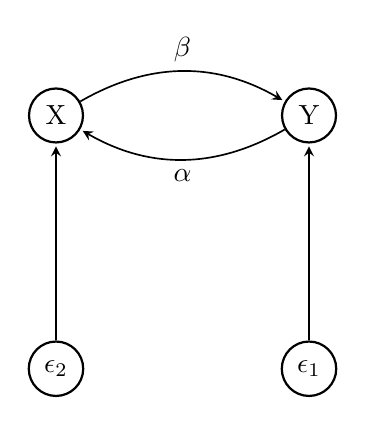
\begin{tikzpicture}[
            > = stealth, % arrow head style
            shorten > = 1pt, % don't touch arrow head to node
            node distance = 2.5cm,% distance between nodes
            semithick, % line style
        ] 
 \tikzstyle{nodestyle}=[
 			 shape = circle,
            draw = black,
            thick,
            fill = white,
            minimum size = 4mm
        ]
\node[nodestyle](X){X};
\node[nodestyle, right=of X](Y){Y};
\node[nodestyle, below=of Y](e1){$\epsilon_1$};
\node[nodestyle, below=of X](e2){$\epsilon_2$};
\path[->, bend left, above] (X) edge node {$\beta$} (Y);
\path[->, bend left, below] (Y) edge node {$\alpha$} (X);
\path[->] (e1) edge (Y);
\path[->] (e2) edge (X);
\end{tikzpicture}

\end{document}
